\documentclass[xcolor=dvipsnames]{beamer}

%%% Packages %%%
\usepackage[utf8]{inputenc}
\usepackage{subfig}
\usepackage{graphicx}
\usepackage{tikz}
\usepackage[absolute, overlay]{textpos}
\usepackage{soul}
\usepackage{booktabs}
\usepackage{multicol}

%%% Creating Tarleton Purple %%%
\definecolor{TarletonPurple}{RGB}{79, 45, 127}


%%% Beamer Theme %%%
\usetheme{PaloAlto}
\usecolortheme[named=TarletonPurple]{structure}


%%% Graphics Path %%%
\graphicspath{{./Images}}

%%% Title Page Info %%%
\title{Synchronization of Chaotic Systems}
\author{David Ebert and Mikaela Jordan}
\institute{Tarleton State University}
\date{February 8, 2017}

%%% Making Reference Environment For Tarleton Picture %%%
\newenvironment{reference}[2]{
\begin{textblock*}{\textwidth}(#1,#2)              
  \footnotesize\it\bgroup\color{red!50!black}}{\egroup\end{textblock*}}


\begin{document}
\makeatletter
\def\beamer@framenotesbegin{
\begin{reference}{1mm}{1mm}
\tikz\node[opacity=0.8]{\includegraphics[scale=0.25]{images/Tarleton_State_University}};
\end{reference} 
}

\frame{\titlepage}

\begin{frame}
	\frametitle{Aggregation}
	\textbf{Definition:}
	\begin{center}
		Grouping coupled objects (typically animals)	
	\end{center}
	\textbf{Examples:}
	\begin{center}
		\begin{itemize}
			\item Flocks of birds
			\item Herds of animals
			\item Schools of fish
			\item Swarms of insects
		\end{itemize}
	\end{center}

\end{frame}

\begin{frame}
	\frametitle{Human Swarming Version I}
	\begin{multicols}{2}
	\begin{itemize}
	\item The Setup:
	\item The Rules:	
		\begin{itemize}
			\item \textbf{Walk} slowly toward center of the group.
			\item \textbf{Slow down} if you're within two feet of another person.
			\item \textbf{Stop} if you are within one foot of another person.
		\end{itemize}
	\end{itemize}
	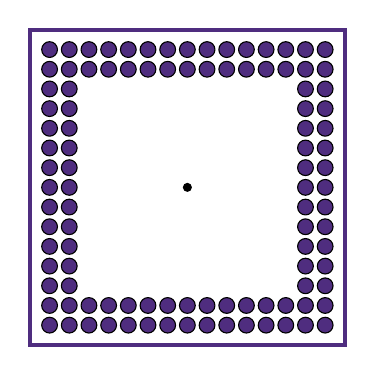
\begin{tikzpicture}
		\draw[ultra thick, TarletonPurple] (0, 0) rectangle (4, 4);
		\foreach \x in {0.25, 0.5, 3.75, 3.5}{
			\foreach \y in {0.25, 0.5, ..., 3.75}{
				\draw[fill=TarletonPurple] (\x, \y) circle (0.1cm);
		}}
		\foreach \x in {0.75, 1.0,..., 3.25}{
			\foreach \y in {0.25, 0.5, 3.75, 3.5}{
				\draw[fill=TarletonPurple] (\x, \y) circle (0.1cm);
			}}
		\draw[fill] (2, 2) circle (0.05cm);
	\end{tikzpicture}
	\end{multicols}
\end{frame}

\begin{frame}
	\frametitle{Human Swarming Version II}
	\begin{multicols}{2}
	\begin{itemize}
	\item The Setup:
	\item The Rules:	
		\begin{itemize}
			\item \textbf{Walk} at a slow, constant speed.
			\item \textbf{Walk} toward the person or people you see in front of you.
			\item \textbf{Turn right} if you are going to collide.
		\end{itemize}
	\end{itemize}
	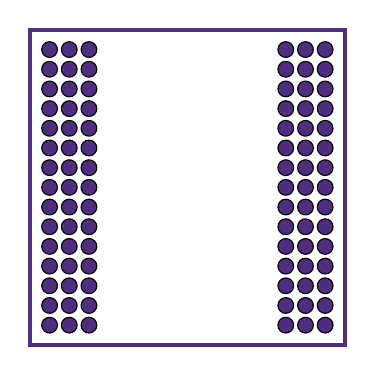
\begin{tikzpicture}
		\draw[ultra thick, TarletonPurple] (0, 0) rectangle (4, 4);
		\foreach \x in {0.25, 0.5, 0.75, 3.75, 3.5, 3.25}{
			\foreach \y in {0.25, 0.5, ..., 3.75}{
				\draw[fill=TarletonPurple] (\x, \y) circle (0.1cm);
		}}
	\end{tikzpicture}
	
	\end{multicols}
\end{frame}

\begin{frame}
	\frametitle{Next Steps}
	\begin{itemize}
		\item Create a better model for Human Swarming I
		\item Create a model for Human Swarming II
		\item Do more research on forces between animal swarms/aggregations
	\end{itemize}
\end{frame}

	
\end{document}
